\documentclass[UTF8]{ctexart}
\usepackage{amsmath}
\usepackage{graphicx}
\usepackage{float}
\usepackage{subfigure}
\usepackage{xeCJK}
\usepackage{hyperref}
\usepackage{algorithm2e}
\usepackage{amsfonts}
\usepackage{epsfig}
\usepackage{listings}
\usepackage{xcolor}
% 定义可能使用到的颜色

\definecolor{CPPLight}  {HTML} {686868}
\definecolor{CPPSteel}  {HTML} {888888}
\definecolor{CPPDark}   {HTML} {262626}
\definecolor{CPPBlue}   {HTML} {4172A3}
\definecolor{CPPGreen}  {HTML} {487818}
\definecolor{CPPBrown}  {HTML} {A07040}
\definecolor{CPPRed}    {HTML} {AD4D3A}
\definecolor{CPPViolet} {HTML} {7040A0}
\definecolor{CPPGray}  {HTML} {B8B8B8}
\lstset{
    columns=fixed,
    numbers=left,                                        % 在左侧显示行号
    frame=none,                                          % 不显示背景边框
    backgroundcolor=\color[RGB]{245,245,244},            % 设定背景颜色
    keywordstyle=\color[RGB]{40,40,255},                 % 设定关键字颜色
    numberstyle=\footnotesize\color{darkgray},           % 设定行号格式
    commentstyle=\it\color[RGB]{0,96,96},                % 设置代码注释的格式
    stringstyle=\rmfamily\slshape\color[RGB]{128,0,0},   % 设置字符串格式
    showstringspaces=false,                              % 不显示字符串中的空格
    language=c++,                                        % 设置语言
    morekeywords={alignas,continute,friend,register,true,alignof,decltype,goto,
    reinterpret_cast,try,asm,defult,if,return,typedef,auto,delete,inline,short,
    typeid,bool,do,int,signed,typename,break,double,long,sizeof,union,case,
    dynamic_cast,mutable,static,unsigned,catch,else,namespace,static_assert,using,
    char,enum,new,static_cast,virtual,char16_t,char32_t,explict,noexcept,struct,
    void,export,nullptr,switch,volatile,class,extern,operator,template,wchar_t,
    const,false,private,this,while,constexpr,float,protected,thread_local,
    const_cast,for,public,throw,std},
}

\graphicspath{{images/}}
\setCJKmonofont{Microsoft YaHei}

\title{\Huge{数学建模实验报告}}
\author{\Huge{易凯}}
\date{\Huge{2017年4月16日}}

\begin{document}
  \maketitle
  \vspace{35mm}
  \begin{flushright}
  \Large{
    \textbf{班\ \ \ \ \ 级} \makebox[5em][l]{软件53班}

    \textbf{学\ \ \ \ \ 号} \makebox[5em][l]{2151601053}

    \textbf{邮\ \ \ \ \ 箱} \makebox[5em][l]{williamyi96@gmail.com}

    \textbf{联系电话} \makebox[5em][l]{13772103675}

    \textbf{个人网站} \makebox[5em][l]{https://williamyi96.github.io}

    \textbf{提交日期} \makebox[5em][l]{2017年4月30日}
    }
    \end{flushright}
    \newpage
    \tableofcontents
    \newpage
    \listoffigures
    \newpage
    \listoftables
    \newpage

    \section{声明}
    此报告为西安交通大学本科生易凯于2017年4月在学习《数学建模》基础之上,加上个人的认识与理解完成的数学建模综合实验报告。未经允许,禁止挪作他用。由于笔者能力有限,而数学模型没有最好只有更好的特性,因此望读者对于其中的缺漏指出能够批评指正。

    \section{微积分的运用--水流出时间}
    \subsection{题目描述}

    \begin{figure}[!htb]
	\centering
	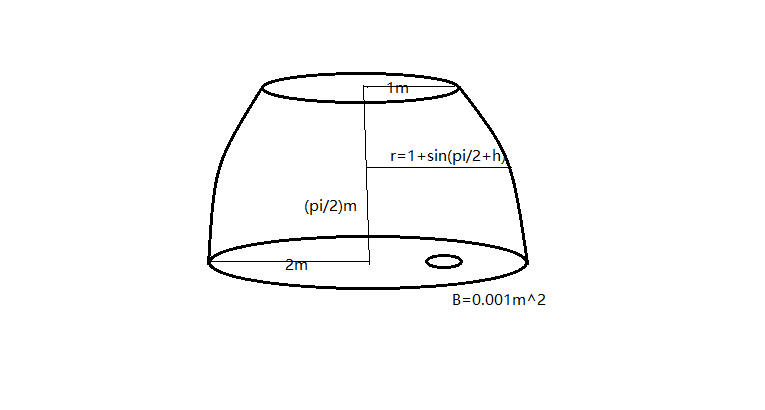
\includegraphics[width=1.0\textwidth]{数学建模第一题图.png}
	\end{figure}

    如图所示,该容器为一个圆台,上底面的半径为1m,下底面的半径为2m,总的高度为$(\pi/2)m$,容器中间的任意一处的半径满足$r=1+sin(\pi/2)+h$。池底有一个横截面积为0.001平方米的圆孔防水,当初始时水池内装满水,水总小孔中流出的速度$v=\sqrt{2gh}$。问将水完全放完所需要花费的时间?(请利用计算机仿真的方法进行求解)

    \subsection{题目分析}
    此为微积分背景之下,数学建模的实践与运用。因此可以建立一个微分方程模型来实现问题的求解。

    \subsection{问题求解}
    我们建立微分方程模型,假设当时间t时水的高度为h,当$t+\Delta{t}$时刻,水面的高度$h+\Delta{h}$,其中$\Delta{h}<0$。

    我们此处依据的原理是:当由t时刻水位降到$t+\Delta{t}$时刻水位时,失去的水量等于从小孔中流出的水量,容易看出的是,从t时刻水位降到$t+\Delta{t}$时刻水位所失去的体积在数量上是$\int_{h}^{h+\Delta{h}}\pi r^2 dh$,当$\Delta t$趋近于0时,实际失去的水量为-$\int_{h}^{h+\Delta{h}}\pi r^2 dt$;在同样的时间里,水从小孔流出的体积是$B\Delta S$, 其中$\Delta S$是水在$\Delta t$时间内从小孔流出的距离。

    由此可见数学的求解实际上相对而言较为复杂,但是如果使用数学仿真的方式则可以较大程度地减小计算量以及思考的难度。

    \subsection{程序代码}
    由于mathematica收费太高,因此使用相对物美价廉的MATLAB进行代码实现。

\begin{lstlisting}[language=matlab]
clear; clc; clf;
grid
hold on
axis([0,6000,0,2])
dt = 0.1;  % 步长设置为t=0.1s
t = 0;
b = 0.001;
g = 9.8;
h = pi/2;  % 初始水位为h
while h >= 0.001    % 当h <= 0.001时认为容器中的水已经全部漏尽
    v = sqrt(2*g*h);
    h = h - b*v*dt/(pi*((1+sin(pi/2+h))*sin(pi/2+h)));
    t = t + dt;
    plot(t, h, 'b.', 'markersize', 3)
end;
fprintf('t=%.0f\n', t)
\end{lstlisting}

该程序仿真之后得到的时间与水位高度的图像为:

\begin{figure}[!htb]
  \centering
  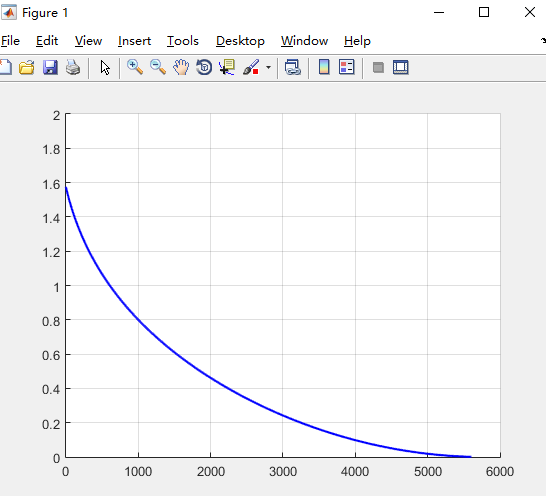
\includegraphics[width=1.0\textwidth]{figure1.png}
  \caption{水流出时间问题的t-h图}\label{水流出时间问题的t-h图}
\end{figure}

最后得到水的流出时间为5595s。

对于计算机的性能以及程序的复杂度得到的运行数据图为:

\begin{figure}[!htb]
  \centering
  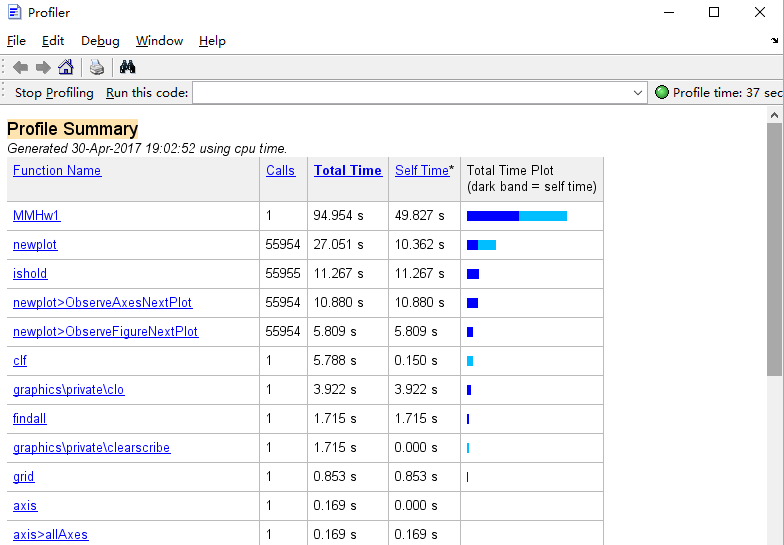
\includegraphics[width=1.0\textwidth]{time1.png}
  \caption{TimeAnalysisOne}\label{TimeAnalysisOne}
\end{figure}

    \subsection{反思总结}
    该题是微积分在水的流出问题中的应用,相对而言在微积分中具有较高的典型性,虽然不是太难,但是求解的思路本身需要遵循高等数学的相关基础性原则,同时针对实际问题提出合适的模型,并根据模型进行求解。

    自己在完成这个题目的题解过程中,发现存在着许多看似差条件的地方,而这也恰恰构成了数学建模的根本魅力之所在,做出合理的假设比单纯地使用某种方法解决特定的问题更加有效。

    \section{最优化问题--资源配置}
    \subsection{题目描述}
    有ABC三个场地,每个场地出产一定量的原料,同时也消耗一定量的产品。具体数据如下表所示。已知制成每吨产品需要消耗三吨原料。ABC距离如图所示。假设每万吨原料运输1km的运费为5000元,每万吨产品运输1km的运费为6000元。由于地区条件的差异,在不同地区设厂的费用不同,由于条件的限制,在B处建厂的规模不能超过5万吨。问:在这三地如何建厂,规模建多大才能使总费用最少?

    \begin{table}
      \centering
      \begin{tabular}{|c|c|c|c|}
        \hline
        % after \\: \hline or \cline{col1-col2} \cline{col3-col4} ...
        地点 & 年产原料(万吨) & 年销产品(万吨) & 生产费用(万元) \\
        \hline
        A & 20 & 7 & 150 \\
        \hline
        B & 16 & 13 & 120 \\
        \hline
        C & 24 & 0 & 100 \\
        \hline
      \end{tabular}
      \caption{各厂原料产品进出一览表}\label{各厂原料产品进出一览表}
    \end{table}

    \begin{figure}[!htb]
	\centering
	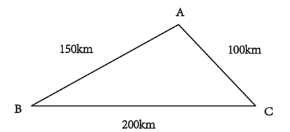
\includegraphics[width=0.8\textwidth]{数学建模第二题图.png}
	\end{figure}

    \subsection{题目分析}
    该题目是典型的最优化问题,解题的基本思路是合理化地设出各个需要优化的未知量,同时找到充分的约束条件进行最小值的求解。

    \subsection{问题求解}
    设A厂建厂的规模为每年生产产品P万吨,B厂建厂的规模为每年生产Q万吨,C厂建厂的规模为每年生产R万吨。

    A厂向B厂每年运送原料ab万吨,向C厂每年运送原料为ac万吨;B厂向A厂每年运送原料ba万吨,向c厂每年运送原料bc万吨;C厂向A厂每年运送原料ca万吨,C厂向B厂每年运送原料cb万吨;

    A厂向B厂每年运送产品xy万吨,向C厂每年运送产品为xz万吨;B厂向A厂每年运送产品为yx万吨,向C厂每年运送产品为yz万吨;C厂向A厂每年运送产品为zx万吨,向B厂每年运送产品为zy万吨。

    \paragraph{最优化目标为:}

    ~

    W = 150P + 120Q + 100R + 75ab + 50ac + 75ba + 100bc + 50ca + 100cb + 90xy + 60xz + 90yx + 120yz + 60zx + 120zy

    \paragraph{最优化条件为:}

    ~

    \subparagraph{1. 不可能将产品和原料运输超过两次}

    \subparagraph{2. 运输量均为正值}

    \subparagraph{3. 经过运输后,每个地方产品量等于销量}

    \subparagraph{4. 由于C地不可销售,因此将C的原料尽可能多地运往外地,同时产品不可运往C}

    ~

    \textbf{则有如下形式化的最优化条件:}

    \begin{lstlisting}[language=c]
    xz = yz = 0
    P + Q + R = 20
    
    ab + ac <= 20
    ba + bc <= 16
    ca + cb <= 24
    
    P - xy >= 0
    Q - yx >= 0
    P - xy + yx + zx = 7
    Q - yx + xy + zy = 13
    R - zx - zy = 0
    
    P >= 0
    Q >= 0
    R >= 0
    ab >= 0
    ac >= 0
    bc >= 0
    ba >= 0
    ca >= 0
    cb >= 0
    xy >= 0
    yx >= 0
    zx >= 0
    zy >= 0
    
    Q <= 5

    3P - ba - ca - 20 + ab + ac = 0
    3Q - ab - cb - 16 + ba + bc = 0
    3R - ac - bc - 24 + ca + cb = 0
    \end{lstlisting}

    \subsection{程序代码}
\begin{lstlisting}[language=matlab]
Minimize[150*P + 120*Q + 100*R + 
            75*ab + 50*ac + 75*ba + 100*bc + 50*ca + 100*cb + 
            90*xy + 60*xz + 90*yx + 120*yz + 60*zx + 120*zy, 
            {xy=0, yz=0, P+Q+R=20, ab + ac <= 20,ba+bc<=16; ca+cb<=24,
                P-xy>=0, Q-yx>=0, 
                P-xy+yx+zx=7, Q-yx+xy+zy=13, R-zx-zy=0, 
                P>=0, Q>=0, R>=0, 
                ab>=0, ac>=0, bc>=0, bc>=0, ba>=0; ca>=0, cb>=0,
                xy>=0, yx>=0, zx>=0, zy>=0,
                Q<=5,
                3*P - ba - ca - 20 + ab + ac = 0,
                3*Q - ab - cb - 16 + ba + bc = 0,
                3*R - ac - bc - 24 + ca + cb = 0},
            {P,Q,R,ab,ac,ba,bc,ca,cb,xy,xz,yx,yz,zx,zy}]
\end{lstlisting}

    \subsection{反思总结}
    通过分析程序的运行结果我们可以得到:

    通过上述的分析基本实现了该问题的求解,但是过程中出现了一些设置上的bug,因此在之后的学习过程中要特别注意。

    \section{随机模型--货物的最优补充}
    \subsection{题目描述}
    某企业对于某种材料的月需求量为随机变量,具有如下表所示的概率分布:
    \begin{table}[!htb]
      \centering
      \begin{tabular}{|c|c|c|c|c|c|c|c|c|}
        \hline
        % after \\: \hline or \cline{col1-col2} \cline{col3-col4} ...
        需求量(吨) & 50 & 60 & 70 & 80 & 90 & 100 & 110 & 120 \\
        \hline
        P(u=j) & 0.10 & 0.20 & 0.15 & 0.25 & 0.05 & 0.10 & 0.10 & 0.05 \\
        \hline
      \end{tabular}
      \caption{对于某种材料的月需求量}\label{对于某种材料的月需求量}
    \end{table}

    每次订货费为500元,每月每吨保管费为50元,每月每吨货物缺货费为1500元,每吨材料的购价为1000元,该企业欲采用周期性盘点的(s,S)策略来控制库存量,求最佳的s和S的值。
    ((s,S)策略指的是若发现存货量少于s时立即补货,当存货补充到S时,使得经济效益最大。)

    \subsection{题目分析}
    该题为典型的贮存模型加上随机化模型的题目,解题的思路是通过计算机仿真的方法来对相关量进行分析,拟合找到使经济效益最大化的(s,S)值。
    \subsection{问题求解}
    该问题的求解思路如下:
    \paragraph{1. 变量初始化操作}
    设置need,remain,cost,min\_cost\_avg等变量分别表示需求量,剩余量,成本,以及最小化成本;

    \paragraph{2. 使用for循环进行计算机模拟}
    分别为s和S设置不同的步长,然后执行100000次找到最优解,思路是生成随机数m,m的范围来确定需求量的范围,然后分析是有剩余还是有缺货,根据相关公式计算成本;

    \paragraph{3. 将计算的100000此的成本值进行平均} 得出对应s与S之下的成本

    \paragraph{4. 通过遍历比较判断得到最优化的成本} 也就是通过简单的比较规则来实现成本最小化结果记录,并进行输出。
    \subsection{程序代码}
\begin{lstlisting}[language=matlab]
clear;clc;clf;
need=0;
remain=0;
cost=0;
min_cost_avg=inf;
for s=30:2:70;
    for S=80:2:140;
        for num=1:100000;
            m=rand;
            if m<=0.1
                need=50;
            elseif m<=0.3
                need=60;
            elseif m<=0.45
                need=70;
            elseif m<=0.7
                need=80;
            elseif m<=0.75
                need=90;
            elseif m<=0.85
                need=100;
            elseif m<=0.95
                need=110;
            else
            need=120;
            end

            if remain<s
                cost=cost+(S-remain)*1000+500;
            if S<need
                cost=cost+(need-S)*1500;
                remain=0;
            else
                cost=cost+(S-need)*50;
                remain=S-need;
            end
            else
            if remain<need
                cost=cost+(need-remain)*1500;
                remain=0;
            else
                cost=cost+(remain-need)*50;
                remain=remain-need;
            end
            end
        end
        cost_avg=cost/100000;
        if cost_avg<min_cost_avg
            min_cost_avg=cost_avg;
            avg_s=s;
            avg_S=S;
        end
        fprintf('s=%d, S=%d\nThe monthly average 
        	cost=%.1f\n',s,S,cost_avg);
        cost=0;
    end
end
fprintf('\nWhen s=%d, S=%d\nThe least monthly average 
	cost=%.1f\n',avg_s,avg_S,min_cost_avg);
\end{lstlisting}

    \subsection{实验结果}
	\begin{figure}
	\centering
	\begin{minipage}[c]{0.5\textwidth}
	\centering
	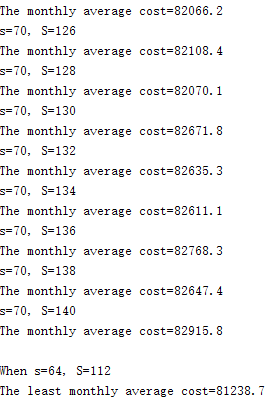
\includegraphics[height=8.5cm,width=5.5cm]{3.1.PNG}
	\end{minipage}%
	\begin{minipage}[c]{0.5\textwidth}
	\centering
	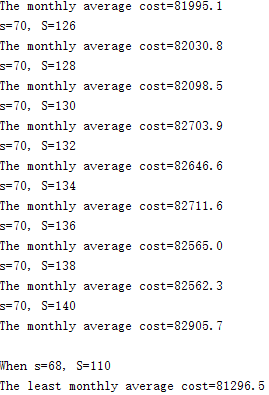
\includegraphics[height=8.5cm,width=5.5cm]{3.2.PNG}
	\end{minipage}
	\caption{贮存模型实验结果I}
	\end{figure}

	\begin{figure}
	\centering
	\begin{minipage}[c]{0.5\textwidth}
	\centering
	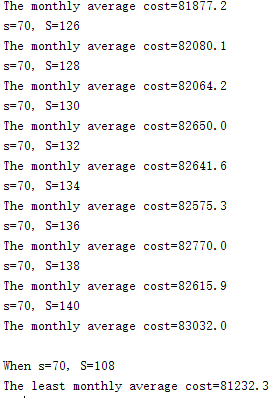
\includegraphics[height=8.5cm,width=5.5cm]{3.3.PNG}
	\end{minipage}%
	\begin{minipage}[c]{0.5\textwidth}
	\centering
	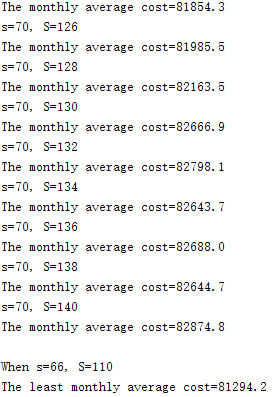
\includegraphics[height=8.5cm,width=5.5cm]{3.4.PNG}
	\end{minipage}
	\caption{贮存模型实验结果II}
	\end{figure}

    \subsection{反思总结}
    该实验是一个将贮存模型与随机模型结合起来的典型实例,通过数学模拟的方法,我们可以从结果以及性能的角度得到较好的模型。这是之后值得注意,并且继续引申的地方。

    \section{综合最优化问题}
    \subsection{题目描述}
    如图所示,27个立方体空盒排成3*3*3的三维阵列。如果三个盒子在同一条水平线上,或者同一条垂直线上,或者同一条对角线上,则认为三盒一线,满足条件的盒子共有49条。
    现有白球13个,黑球14个,每个盒子放入一个球,如果投放,能使有单一色球的线数最少。

    \begin{figure}[!htb]
	\centering
	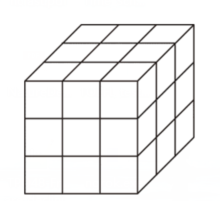
\includegraphics[width=0.8\textwidth]{数学建模第四题图.png}
	\end{figure}

    \subsection{题目分析}
    将该问题的数学化表述就是将黑球形象地记为1,而将白球形象记为0,同时如果黑球三球一线,那么sum的值+3,如果白球三球一线,那么sum的值+0,最后计算出单一色球的线数最小值。

    \subsection{问题求解}
    问题求解的总体思路参见题目分析,问题求解的具体化分析参见源代码。

    \subsection{程序代码}
    \begin{lstlisting}[language=matlab]
for num=1:10000
    n=0;
    for ch=1:10000
        t=0;
        for i=1:3
            for j=1:3
                for k=1:3
                    f(i,j,k)=randi(1);
                    t=t+f(i,j,k);
                end
            end
        end
        if t==13     
            break;
        end
    end
    for i=1:3
        for j=1:3
            for k=1:3
                if sum(f(i,j,:))==3||sum(f(i,j,:))==0
                	||sum(f(:,j,k))==3||sum(f(:,j,k))==0
                	||sum(f(i,:,k))==3||sum(f(i,:,k))==0
                    n=n+1;
                end
            end
        end
    end
    for k=1:3
        if f(1,1,k)==f(2,2,k)&&f(1,1,k)==f(3,3,k)
            n=n+1;
        elseif f(3,1,k)==f(2,2,k)&&f(3,1,k)==f(1,3,k)
            n=n+1;
        end
    end
    for i=1:3
        if f(i,1,1)==f(i,2,2)&&f(i,1,1)==f(i,3,3)
            n=n+1;
        elseif f(i,1,3)==f(i,2,2)&&f(i,1,3)==f(i,3,1)
            n=n+1;
        end
    end
    for j=1:3
        if f(1,j,1)==f(2,j,2)&&f(1,j,1)==f(3,j,3)
            n=n+1;
        elseif f(3,j,1)==f(2,j,2)&&f(3,j,1)==f(1,j,3)
            n=n+1;
        end
    end
    tmp=0;
    for i=1:2:3
        for j=1:2:3
            for k=1:2:3
                if f(i,j,k)+f(4-i,4-j,4-k)==2*f(2,2,2)
                    tmp=tmp+1;
                end
            end
        end
    end
    n=n+tmp/2;
    less(num)=n;
    g(:,:,:,num)=f;
    if num>1
        if less(num)>less(num-1)
            g(:,:,:,num)=g(:,:,:,num-1);
            less(num)=less(num-1);
        end
    end
end
less(num)
g(:,:,:,num)
    \end{lstlisting}

    该程序运行的结果为:
    \begin{lstlisting}[language=matlab]
    	ans =

	4

	ans(:,:,1) =
	1 0 1

	0 1 0

	1 0 1

	ans(:,:,2) =

	0 1 1

	1 0 0

	0 0 1

	ans(:,:,3) =

	0 1 0

	0 0 1

	1 1 0
    \end{lstlisting}

    从实验结果可以看到,单一色球线数最少为4,同时球的排列如上图ans所示,ans(:,:,i)表示立方体的第i层的排布情况。

    \subsection{反思总结}
    该实验是一个综合最优化的问题,我们通过仿真的方法可以较为直观地得到结果。同时,需要注意在进行实际问题数学化处理时,我们将黑球记为1,白球记为0的操作可以进一步拓展。

    \section{理发店服务过程仿真}
    \subsection{题目描述}
    一个理发店有10位服务员A1,A2,...,A10,顾客随机地到达该理发店,每分钟有一个顾客到达,两个顾客到达和没有顾客到达的概率分别为1/2,1/8,3/8,。其中每个顾客的理发时间是随机的,服从均值为15,方差为4的正态分布。试对该理发店一个工作日的情况进行仿真,给出服务员的工作效率和顾客的平均等待时间。

    \subsection{题目分析}
    该题目是在随机模型之下对于数学建模的概念及其相关方法的考察,因此其建立与随机模型的思路基本一致。

    \subsection{问题求解}
    以下采用计算机仿真的方式对于理发店服务过程问题进行求解。步骤如下:

    \paragraph{初始化}  将MATLAB以及各个变量进行初始化

    \paragraph{开始执行循环,解决如下问题:}

    ~

    \textbf{1. 是否有顾客来到}

    \textbf{2. 每个顾客的理发时间}

    \textbf{3. 每个服务员的状态}

    \textbf{4. 排队情况的处理}

    \textbf{5. 排队时间累加}

    \textbf{6. 求平均,得出时间}

    在求解的过程中,根据查表结果在仿真过程中将正态分布进行数据化。

    \subsection{程序代码}
    \begin{lstlisting}[language=matlab]
	    % 进行相关初始化
	clc;clear;
	a(10)=0;
	b(10)=0;
	s=0;w=0;

	% 循环仿真
	for minute=1:480
	    m=rand;
	    if m<=0.001
	        h=8.5;
	    elseif m<=0.006
	        h=9.5;
	    elseif m<=0.023
	        h=10.5;
	    elseif m<=0.067
	        h=11.5;
	    elseif m<=0.159
	        h=12.5;
	    elseif m<=0.308
	        h=13.5;
	    elseif m<=0.5
	        h=14.5;
	    elseif m<=0.692
	        h=15.5;
	    elseif m<=0.841
	        h=16.5;
	    elseif m<=0.933
	        h=17.5;
	    elseif m<=0.977
	        h=18.5;
	    elseif m<=0.994
	        h=19.5;
	    elseif m<=0.999
	        h=20.5;
	    else
	        h=21.5;
	    end
	    
	    n=rand;
	    if n<=0.5
	        s=s+1;
	        min=inf;jj=0;
	        for j=1:10
	            if a(j)<min
	                min=a(j);
	                t=j;
	            end
	        end
	        if min<0
	            min=0;
	        end
	        w=w+min;
	        a(t)=a(t)+h;
	    elseif n<=0.625
	        s=s+2;
	        mm=rand;
	        if mm<=0.001
	            hh=8.5;
	        elseif mm<=0.006
	            hh=9.5;
	        elseif mm<=0.023
	            hh=10.5;
	        elseif mm<=0.067
	            hh=11.5;
	        elseif mm<=0.159
	            hh=12.5;
	        elseif mm<=0.308
	            hh=13.5;
	        elseif mm<=0.5
	            hh=14.5;
	        elseif mm<=0.692
	            hh=15.5;
	        elseif mm<=0.841
	            hh=16.5;
	        elseif mm<=0.933
	            hh=17.5;
	        elseif mm<=0.977
	            hh=18.5;
	        elseif mm<=0.994
	            hh=19.5;
	        elseif mm<=0.999
	            hh=20.5;
	        else
	            hh=21.5;
	        end
	        
	        for j=1:10
	            if a(j)<min
	                min=a(j);
	                t=j;
	            end
	        end
	        if min<0
	            min=0;
	        end
	        w=w+min;
	        a(t)=a(t)+h;
	        for j=1:10
	            if a(j)<min
	                min=a(j);
	                t=j;
	            end
	        end
	        if min<0
	            min=0;
	        end
	        w=w+min;
	        a(t)=a(t)+hh;
	    end
	    for j=1:10
	        if a(j)>0
	            a(j)=a(j)-1;
	        else
	            b(j)=b(j)+1;
	        end
	    end
	end
	for j=1:10
	    1-b(j)/480
	end
	w=w/s
	s
    \end{lstlisting}

   	运行上述代码,得到的结果如下所示:

   	\begin{figure}
	\centering
	\begin{minipage}[c]{0.3\textwidth}
	\centering
	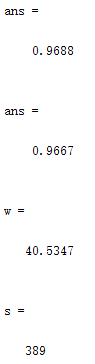
\includegraphics[height=8.5cm,width=2.0cm]{5.1.PNG}
	\end{minipage}%
	\begin{minipage}[c]{0.3\textwidth}
	\centering
	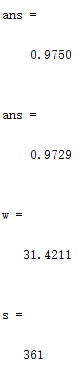
\includegraphics[height=8.5cm,width=2.0cm]{5.2.PNG}
	\end{minipage}
	\begin{minipage}[c]{0.3\textwidth}
	\centering
	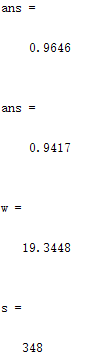
\includegraphics[height=8.5cm,width=2.0cm]{5.3.PNG}
	\end{minipage}
	\caption{理发店仿真结果}
	\end{figure}

	其中ans即为员工的工作效率,w/s即为平均等待时间(以分钟计算)。
    
    \subsection{反思总结}

    \section{收获总结}
    半个学期的《数学建模》课程的学习就这样结束了,同时也是戴老师交给我们的最后一次课了,大一的时候,高等数学的任课老师,对于我之后的学习发展产生了较为深远的影响,而当我大二时由于参加了多个竞赛以及进行科研训练,包括其他课程的学业压力,再也没有时间像大一一样再去将一个问题去穷根问底了,但是这为其十余周的数学建模的学习仍然让我收获良多,感慨良多。

   	我将从\textbf{能力提升},\textbf{意识培养},\textbf{认识不足},\textbf{兴趣提升},\textbf{注重想法},\textbf{敢于开拓}这六个角度进行归纳总结:

   	\subsection{能力提升}
   	学习数学建模的过程中,让我第一次觉得将一个自然物抽象之后建立数学模型并不是一件很难的事情,同时数学模型本身就存在于我们生活的方方面面,就像质点,直线等等,在建模的学习过程中发现自我的抽象能力得到了较大的提升。

   	\subsection{意识培养}
   	戴老师上课反复强调,数学建模培养的是大家的能力,是大家的按照建模流程进行分析问题,解决问题的意识,这种意识才是比知识更为重要的东西。老师在课堂之上循循善诱,逐步地引导我们这个模型是怎样建立起来的,同时又会经历哪些修正,同时又是如何去提升模型的性能。在这个过程中,培养了自己的数学建模的分析意识。

   	\subsection{认识不足}
   	在建模课程的学习过程中,这段经历总体而言是非常有趣的,很多的老师精选的例题不仅具有代表性,同时不乏趣味性,让我打开眼界,原来,有时候数学还可以这样用,原来实际问题可以用这么普通但是这么实用的方式去解决问题。

   	在完成实验报告的过程中,总体思路还是挺顺畅的,但是实际地单独对于某些问题进行系统分析的过程之中,发现实际上遇到了一些阻碍,同时也说明了自己的能力有待提升。看到课外拓展的一些题,更具有挑战性,之后要加强这方面能力的提升以及强化训练。

   	\subsection{兴趣提升}
   	数学建模个人认为更多的就是将数学进行运用来解决实际问题的一个过程,在这个过程中,遇到了很多新奇有趣的题目,同时也运用了许多让人眼前一亮的方法,极大地提升了自己进一步学习数学建模,并提升建模能力的兴趣。

   	\subsection{注重想法}
   	数学建模或者说数学模型的核心在于做出合理化的假设,往往假设的好坏决定了模型的好坏,因此需要敢于去提出自己的想法,然后不断地修正,以期臻于完美。

   	\subsection{敢于开拓}
   	数学模型的一个很重要的原则是,没有最好,只有更好,因此只有不断地去修正,不断地去开拓创新,才能够不断地提升模型的性能。

   	同时,其他课程以及科研训练的真谛也在于此,真正的魅力不在于我马上就可以找到解决问题的最好方法,而是在不断地摸索中,提升了个人的能力,培养了开拓创新的精神,这才是社会赖以生存发展的本质意义。

    \section{致谢}
    Give my sincere thanks to Teacher Dai for his excellent teaching skills and serious altitude for our homework. Give my sincere thanks to some students who have helped me and who have inspired me when discussing with them. Give my sincere thanks to myself because I've overcome all difficulties and have successfully finished my math modeling assignments. Give my sincere thanks to those pioneers who have devoted themselves to writing immortal books. Give my sincere thanks to all the people sharing their ideas and harvests without pay in QA communities.

    衷心感谢戴永红老师出色的教学风范以及严谨的治学态度,衷心感谢那些在讨论中帮助和启发我的同学们,衷心感谢克服了种种困难最终完成了数学建模作业的自己,衷心感谢那些写了不朽著作为后人指明道路的先驱们,衷心感谢那些在问答社区无私奉献自己智慧成果的所有同仁!

    \section{参考文献}
    [1] 周义仓,赫孝良. 《数学建模实验》[M].第二版. 西安:西安交通大学出版社. 2016-12.

    [2] 戴永红. 《数学建模系列课件》. 西安:西安交通大学. 2017年春.

    [3] Frank R.Giordano,Maurice D.Weir,William P.Fox. 《数学建模》[M]. 机械工业出版社. 2004-1.

    [4] 米尔斯切特. 《数学建模方法与分析》[M]. 机械工业出版社. 2005-6.

    [5] 姜启源. 《数学模型》[M]. 高等教育出版社. 2006-1.

    %\begin{thebibliography}{123456}
    %\bibitem {JW1}周义仓,赫孝良. 《数学建模实验》[M].第二版. 西安:西安交通大学出版社. 2016-12.
    %\bibitem {JW2}戴永红. 《数学建模系列课件》. 西安:西安交通大学. 2017年春.
    %\bibitem {JW3}Frank R.Giordano,Maurice D.Weir,William P.Fox. 《数学建模》[M]. 机械工业出版社. 2004-1.
    %\bibitem {JW4}米尔斯切特. 《数学建模方法与分析》[M]. 机械工业出版社. 2005-6.
    %\bibitem {JW5}姜启源. 《数学模型》[M]. 高等教育出版社. 2006-1.
    %\end{thebibliography}

\end{document} 